\chapter{Линии связи}

\textbf{\textit{Линия связи}} в общем случае состоит из:
\begin{itemize}
    \item физической среды, по которой передаются электрические (оптические) информационные сигналы;
    \item аппаратуры передачи данных;
    \item промежуточной аппаратуры.
\end{itemize}

Синонимом термина линия связи (line) в нашем изложении является термин канал связи (channel).

\section{Типы линий связи. Физическая среда передачи данных}

\textbf{\textit{Физическая среда передачи данных (medium)}} может представлять собой кабель, т.е. набор проводников, изоляционных и защитных оболочек и соединительных разъемов, а также земную атмосферу или космическое пространство, через которые распространяются электромагнитные волны.

В зависимости от среды передачи данных линии связи разделяются на следующие:
\begin{itemize}
    \item проводные (воздушные);
    \item кабельные (медные и волоконно-оптические);
    \item радиоканалы наземной и спутниковой связи.
\end{itemize}

\begin{figure}
    \centering
    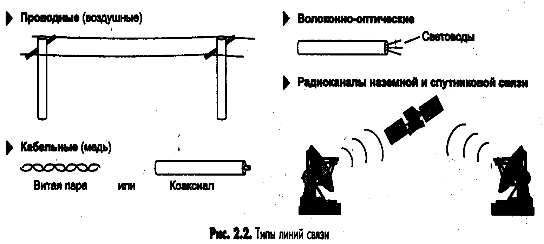
\includegraphics[width=0.7\textwidth]{wired-lines}
    \caption{Проводные линии связи}
    \label{fig:wired-lines}
\end{figure}

\textbf{\textit{Проводные (воздушные) линии связи}} представляют собой провода без изолирующих или экранирующих оплеток, проложенные между столбами и висящие в воздухе.

По таким линиям связи традиционно передаются телефонные или телеграфные сигналы.
Скоростные качества и помехозащищенность этих линий оставляют желать много лучшего.

\subsection{Кабельные линии}

\textbf{\textit{Кабельные линии}} представляют собой достаточно сложную конструкцию.
Кабель состоит из проводников, заключенных в несколько слоев изоляции - электрической, электромагнитной, механической, а также, возможно, климатической.
Кроме того, кабель может быть оснащен разъемами, позволяющими быстро выполнять присоединение к нему различного оборудования.
В компьютерных сетях применяются три основных типа кабеля:
\begin{itemize}
    \item кабели на основе скрученных пар медных проводов (витые пары);
    \item коаксиальные кабели с медной жилой;
    \item волоконно-оптические кабели.
\end{itemize}

Скрученная пара проводов называется \emph{витой парой (twistedpair)}.
Витая пара существует в экранированном варианте (Shielded Twistedpair, STP), когда пара медных проводов обертывается в металлический экран, и неэкранированном \emph{(Unshielded Twistedpair, UTP)}, когда металлический экран отсутствует.
Скручивание проводов снижает влияние внешних помех на полезные сигналы, передаваемые по кабелю.

\emph{Коаксиальный кабель (coaxial)} состоит из внутренней медной жилы и оплетки, отделенной от жилы слоем изоляции.
Существует различные типы коаксиального кабеля, отличающиеся характеристиками и областями применения.

\emph{Волоконно-оптический кабель (optical fiber)} состоит из тонких (5-60 микрон) волокон, по которым распространяются световые сигналы.
Это наиболее качественный тип кабеля - он обеспечивает передачу данных с очень высокой скоростью (до 10 Гбит/с и выше) и обеспечивает самую лучшую защиту данных от внешних помех.

\subsection{Радиоканалы наземной и спутниковой связи}

\emph{Радиоканалы наземной и спутниковой связи} образуются с помощью передатчика и приемника радиоволн.
Существует большое количество различных типов радиоканалов, отличающихся как используемым частотным диапазоном, так и дальностью канала.

В компьютерных сетях сегодня применяются практически все описанные типы физических сред передачи данных.

Наиболее перспективными являются волоконно-оптические, на которых сегодня строятся как магистрали крупных территориальных сетей, так и высокоскоростные линии связи локальных сетей
Популярной средой является также витая пара, которая характеризуется отличным соотношением качества к стоимости, а также простотой монтажа.
С помощью витой пары обычно подключают конечных абонентов сетей на расстояниях до 100 метров от концентратора.

Спутниковые каналы и радиосвязь используются чаще всего в тех случаях, когда кабельные линии связи применить нельзя - например, при прохождении канала через малонаселенную местность или же для связи с мобильным пользователем сети, таким как шофер грузовика, врач, совершающий обход, и т.п.

\section{Типы линий связи. Аппаратура линий связи}

\subsection{Аппаратура передачи данных}

\emph{Аппаратура передачи данных (АПД или DCE - Data Circuit terminating Equipment)} традиционно входит в состав линии связи и непосредственно связывает компьютеры или локальные сети пользователя с линией связи, являясь, таким образом, пограничным оборудованием.
Обычно DCE работает на физическом уровне, отвечая за передачу и прием сигнала нужной формы и мощности в физическую среду.
Примерами DCE являются модемы, сетевые адаптеры локальных сетей, устройства подключения к цифровым каналам и т.
д.

\emph{Аппаратура пользователя линии связи}, вырабатывающая данные для передачи по линии связи и подключаемая непосредственно к АПД, обобщенно носит название оконечное оборудование данных (ООД или DTE - Data Terminal Equipment).
Примером DTE могут служить компьютеры или маршрутизаторы  локальных сетей.
Эту аппаратуру не включают в состав линии связи.

Разделение оборудования на классы DCE и DTE в локальных сетях является достаточно условным.
Например, адаптер локальной сети можно считать как принадлежностью компьютера, то есть DTE, так и составной частью канала связи, то есть DCE.

\subsection{Промежуточная аппаратура}

Промежуточная аппаратура обычно используется на линиях связи большой протяженности.
Промежуточная аппаратура решает две основные задачи:
\begin{itemize}
    \item улучшение качества сигнала;
    \item создание составного канала связи между двумя абонентами сети.
\end{itemize}

\emph{В локальных сетях} промежуточная аппаратура может не использоваться, если протяженность физической среды позволяет одному сетевому адаптеру принимать сигналы непосредственно от другого без промежуточного усиления.
В противном случае применяются устройства типа \emph{повторителей и концентраторов}.

\emph{В глобальных сетях} необходимо обеспечить качественную передачу сигналов на расстояния в сотни и тысячи километров.
Поэтому без \emph{усилителей сигналов}, установленных через определенные расстояния, построить территориальную линию связи невозможно.
В глобальной сети необходима также и промежуточная аппаратура другого рода - \emph{мультиплексоры, демультиплексоры и коммутаторы}.
Эта аппаратура решает вторую указанную задачу, то есть создает между двумя абонентами сети составной канал из отрезков физической среды - кабелей с усилителями.

Промежуточная аппаратура канала связи прозрачна для пользователя, он ее не замечает и учитывает в своей работе только качество канала, влияющее на скорость передачи дискретных данных.
В действительности же промежуточная аппаратура образует сложную сеть (первичную), которая никаких высокоуровневых служб не поддерживает, а только служит основой для построения компьютерных, телефонных или иных сетей.

\subsection{Аналоговые и цифровые линии связи}

В зависимости от типа промежуточной аппаратуры все линии связи делятся на \emph{аналоговые и цифровые}.

В \emph{аналоговых линиях} промежуточная аппаратура предназначена для усиления аналоговых сигналов, т.е.
сигналов, которые имеют непрерывный диапазон значений.
При аналоговом подходе обычно используется техника частотного мультиплексирования (Frequency Division Multiplexing, FDM).

В \emph{цифровых линиях} связи передаваемые сигналы имеют конечное число состояний.
С помощью таких сигналов передаются как компьютерные данные, так и оцифрованные речь и изображение.
В цифровых каналах связи используется промежуточная аппаратура, которая улучшает форму импульсов за счет их регенерации (восстановления).
Промежуточная аппаратура цифровых каналов работает по принципу временного мультиплексирования каналов (Time Division Multiplexing, TDM).

\section{Характеристики линий связи}

\subsection{Типы характеристик и способы их определения}

К основным характеристикам линий связи относятся:
\begin{itemize}
    \item амплитудно-частотная характеристика (ширина полосы пропускания, затухание);
    \item пропускная способность;
    \item помехоустойчивость;
    \item перекрестные наводки на ближнем конце линии;
    \item достоверность передачи данных;
    \item удельная стоимость.
\end{itemize}

В первую очередь важны такие характеристики, как пропускная способность и достоверность передачи данных, поскольку именно они определяют производительность и надежность создаваемой сети.

\subsection{Амплитудно-частотная характеристика линии}

Степень искажения синусоидальных сигналов линиями связи оценивается с помощью понятия \emph{амплитудно-частотной характеристики} - зависимости коэффициента передачи от частоты.
Знание амплитудно-частотной характеристики реальной линии и спектра входного сигнала позволяет определить спектр выходного сигнала путем вычисления произведения спектра входного сигнала и амплитудно-частотной характеристики.

\subsection{Ширина полосы пропускания и затухание}

На практике вместо амплитудно-частотной характеристики применяются другие, усредненные характеристики – \emph{ширина полосы пропускания и затухание}.

\emph{Ширина полосы пропускания (bandwidth)} - это область частот, в пределах которой нормированное по максимальному значению отношение амплитуды выходного сигнала к амплитуде входного сигнала превышает уровень 0,5.

\emph{Затухание (attenuation)} определяется как относительное уменьшение амплитуды или мощности сигнала при передаче по линии сигнала определенной частоты.

\subsection{Условие неискаженной передачи сигнала линией}

Для неискаженной передачи сигнала большое значение имеет совпадение полос частот спектра сигнала и амплитудно-частотной характеристики.

Если \emph{значимые спектральные составляющие сигнала} (т.е. те, которые вносят основной вклад в результирующий сигнал) \emph{попадают в полосу пропускания линии}, то такой сигнал будет хорошо передаваться данной линией связи и приемник сможет правильно распознать информацию, отправленную по линии передатчиком.

Если же значимые спектральные составляющие выходят за границы полосы пропускания линии связи, или полоса пропускания линии связи значительно шире того участка спектра, в котором расположены значимые компоненты спектра сигнала, то сигнал будет значительно искажаться, приемник будет ошибаться при распознавании информации, а значит, информация не сможет передаваться с заданной пропускной способностью.

\emph{Затухание} $A$ обычно измеряется в децибелах (дБ, decibel - dB) и вычисляется по следующей формуле:
\[
    A = 10 \log_{10} \frac{P_\text{вых}}{P_\text{вх}},
\]
где $P_\text{вых}$ - мощность сигнала на выходе, $P_\text{вх}$ - мощность сигнала на входе линии.

Значения затухания являются паспортными данными кабелей и приводятся на рабочих частотах.
Например, кабель на витой паре категории $5$ характеризуется затуханием не ниже $-23,6~дБ$ для частоты $100~МГц$ при длине кабеля $100~м$.

Абсолютный уровень мощности, например, уровень мощности передатчика, также измеряется в децибелах.
При этом значение мощности сигнала, относительно которого измеряется текущая мощность, принимается равным $1~мВт$.
Таким образом, уровень мощности $P$ вычисляется по следующей формуле:
\[
    P = 10 \log_{10} \frac{P}{1~\text{мВт}},
\]
где $Р$ - мощность сигнала в милливаттах, а дБм (dBm) - это единица измерения уровня мощности (децибел на 1 мВт).

Таким образом, амплитудно-частотная характеристика, полоса пропускания и затухание являются универсальными характеристиками, и их знание позволяет сделать вывод о том, как через линию связи будут передаваться сигналы любой формы.

\subsection{Пропускная способность линии}

\emph{Пропускная способность (throughput) линии} характеризует максимально возможную скорость передачи данных по линии связи.
Пропускная способность измеряется в битах в секунду - бит/с, а также в производных единицах, таких как килобит в секунду (Кбит/с), мегабит в секунду (Мбит/с), гигабит в секунду (Гбит/с) и т.д.

Пропускная способность линий связи и коммуникационного сетевого оборудования традиционно измеряется в битах в секунду, а не в байтах в секунду, так как данные в сетях передаются последовательно, то есть побитно, а не параллельно, байтами, как это происходит внутри компьютера.
Такие единицы измерения, как килобит, мегабит или гигабит, в сетевых технологиях строго соответствуют степеням $10$ (то есть килобит - это $1000~бит$, а мегабит - это $1 000 000~бит$), а не близким к этим числам степеням 2, как это принято в программировании, где приставка <<кило>> равна $2^{10}$ - $1024$, а <<мега>> – $2^{20}$ - $1 048 576$.

Пропускная способность линии связи ограничивается частотными свойствами линии связи и зависит не только от характеристик линии связи, но и от способа представления дискретной информации – физического или линейного кодирования.

При физическом кодировании используют изменение какого-либо параметра сигнала.
Если сигнал изменяется так, что можно различить только два его состояния, то любое его изменение будет соответствовать наименьшей единице информации - биту.
Если же сигнал может иметь более двух различимых состояний, то любое его изменение будет нести несколько бит информации.

Количество изменений информационного параметра в секунду измеряется в бодах (baud).
Период времени между соседними изменениями информационного сигнала называется тактом работы передатчика.

Пропускная способность линии в битах в секунду в общем случае не совпадает с числом бод.
Она может быть как выше, так и ниже числа бод, и это соотношение зависит от способа кодирования.

Если сигнал имеет более двух различимых состояний, то пропускная способность в битах в секунду будет выше, чем число бод.
На примере, приведенном на нижней эпюре рисунка информационным параметром является значение амплитуды импульсов, причем допустимыми являются 4 различимых, отличных от нуля значения, соответствующие состояния значения фаза и амплитуда синусоиды, причем различаются 4 состояния фазы в 0, 90, 180 и 270 градусов и два значения 1~В, 0.5~В, -0.5~В, -1~В.
Это позволяет за один такт передать 2 бит информации, т.е. реализовать скорость передачи информации в 2 раза выше, чем при использовании сигнала с двумя разрешенными состояниями информационного параметра.

\begin{figure}
    \centering
    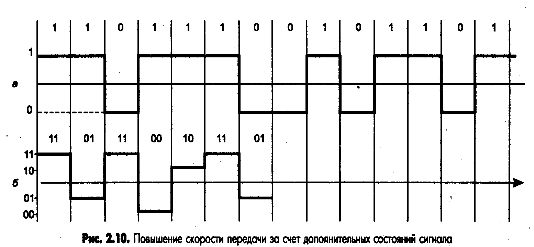
\includegraphics[width=0.7\textwidth]{speed-increasing}
    \caption{Повышение скорости передачи за счёт дополнительных состояний сигнала}
    \label{fig:speed-increasing}
\end{figure}

При использовании сигналов с двумя различимыми состояниями может наблюдаться обратная картина.
Это часто происходит потому, что для надежного распознавания приемником пользовательской информации каждый бит в последовательности может кодироваться несколькими изменениями информационного параметра сигнала.
Например, при кодировании единичного значения бита импульсом положительной полярности, а нулевого значения бита - импульсом отрицательной полярности физический сигнал дважды изменяет свое состояние при передаче каждого бита.
При таком кодировании пропускная способность линии в два раза ниже, чем число бод, передаваемое по линии.

Заметим, что на пропускную способность линии оказывает влияние не только физическое, но и \emph{логическое кодирование}.
Логическое кодирование выполняется до физического кодирования и подразумевает замену бит исходной информации новой последовательностью бит, несущей ту же информацию, но обладающей, кроме этого, дополнительными свойствами, например возможностью для приемной стороны обнаруживать ошибки в принятых данных.
При логическом кодировании чаще всего исходная последовательность бит заменяется более длинной последовательностью, поэтому полезная пропускная способность канала при этом уменьшается.

\subsection{Связь между пропускной способностью линии и ее полосой пропускания}

Связь между отношением сигнал/шум, полосой пропускания линии и ее максимально возможной пропускной способностью, вне зависимости от принятого способа физического кодирования, установил Клод Шеннон:
\[
    C = F \log_2 \left(l + \frac{P_\text{с}}{P_\text{ш}}\right),
\]
где $C$ - максимальная пропускная способность линии в битах в секунду, $F$ - ширина полосы пропускания линии в герцах, $P_\text{с}$ - мощность сигнала, $P_\text{ш}$ - мощность шума.

Из этого соотношения видно, что, хотя теоретического предела пропускной способности линии с фиксированной полосой пропускания не существует, на практике такой предел имеется.
Действительно, повысить пропускную способность линии можно за счет увеличения отношения сигнал/шум - увеличения мощности передатчика или же уменьшения мощности шума (помех) на линии связи, так как влияние мощностей полезного сигнала и шума на пропускную способность ограничено логарифмической зависимостью.
Так, при типовом отношении мощности сигнала к мощности шума в 100 раз повышение мощности передатчика в 2 раза даст только $15~\%$ увеличение пропускной способности линии.

Близким по сути к формуле Шеннона является следующее соотношение, полученное Найквистом:
\[
    C = 2 F \log_2 M,
\]
где $M$ - количество различимых состояний информационного параметра.

Если сигнал имеет 2 различимых состояния, то пропускная способность равна удвоенному значению ширины полосы пропускания линии связи.
Если же передатчик использует более двух устойчивых состояния сигнала для кодирования данных, то пропускная способность линии повышается, так как за один такт работы передатчик передает несколько бит исходных данных, например 2 бита при наличии четырех различимых состояний сигнала.

Хотя формула Найквиста явно не учитывает наличие шума, косвенно его влияние отражается в выборе количества состояний информационного сигнала.
Для повышения пропускной способности канала хотелось бы увеличить это количество \emph{до значительных величин}, но на практике мы не можем этого сделать из-за шума на линии, так как если шум превышает разницу между соседними уровнями, то приемник не сможет устойчиво распознавать передаваемые данные.
Поэтому количество возможных состояний сигнала в формуле Найквиста фактически ограничивается отношением сигнал/шум.

\subsection{Помехоустойчивость и достоверность}

\emph{Помехоустойчивость линии} определяет ее способность уменьшать уровень внешних помех.
Помехоустойчивость линии зависит от типа используемой физической среды, а также от экранирующих и подавляющих помехи средств самой линии.
Наименее помехоустойчивыми являются радиолинии, хорошей устойчивостью обладают кабельные линии и отличной - волоконно-оптические линии, малочувствительные к внешнему электромагнитному излучению.

\emph{Перекрестные наводки на ближнем конце (Near End Cross Talk - NEXT)} определяют помехоустойчивость кабеля к внутренним источникам помех, когда электромагнитное поле сигнала, передаваемого выходом передатчика по одной паре проводников, наводит на другую пару проводников сигнал помехи.
Показатель NEXT, выраженный в децибелах, равен $10 \log \frac{P_\text{вых}}{P_\text{нав}}$, где $P_\text{вых}$ - мощность выходного сигнала передатчика, $Р_\text{нав}$ - мощность наведенного им сигнала на соседнюю пару.

Чем меньше значение NEXT, тем лучше кабель.
Так, для витой пары категории 5 показатель NEXT должен быть меньше -27~дБ на частоте 100~МГц.

Показатель NEXT обычно используется применительно к кабелю, состоящему из нескольких витых пар, так как в этом случае взаимные наводки одной пары на другую могут достигать значительных величин.

В случае, если используется передача данных одновременно по нескольким витым парам, применяется показатель PowerSUM, который отражает суммарную мощность перекрестных наводок от всех передающих пар в кабеле.

\emph{Достоверность} передачи данных характеризует вероятность искажения для каждого передаваемого бита данных.
Иногда этот же показатель называют интенсивностью битовых ошибок (Bit Error Rate, BER).
Величина BER для каналов связи без дополнительных средств защиты от ошибок (например, самокорректирующихся кодов или протоколов с повторной передачей искаженных кадров) составляет, как правило, $10^{–4} – 10^{-6}$, в оптоволоконных линиях связи – $10^{-9}$.
Значение достоверности передачи данных, например, в $10^{-4}$ говорит о том, что в среднем из $10 000~бит$ искажается значение одного бита.

\section{Стандарты кабелей}

Кабель - это достаточно сложное изделие, состоящее из проводников, слоев экрана и изоляции.
В некоторых случаях в состав кабеля входят разъемы, с помощью которых кабели присоединяются к оборудованию.
Кроме этого, для обеспечения быстрой перекоммутации кабелей и оборудования используются различные электромеханические устройства, называемые кроссовыми секциями, кроссовыми коробками или шкафами.

\subsection{Наиболее употребительные стандарты кабельных систем}

В компьютерных сетях применяются кабели, удовлетворяющие определенным стандартам, что позволяет строить кабельную систему сети из кабелей и соединительных устройств разных производителей.
Сегодня наиболее употребительными стандартами в мировой практике являются:
\begin{itemize}
    \item Американский стандарт EIA/TIA-568A, который был разработан совместными усилиями нескольких организаций: ANSI, EIA/TIA и лабораторией Underwriters Labs (UL).
        Стандарт EIA/TIA-568А разработан на основе предыдущей версии стандарта EIA/TIA-568 и дополнений к этому стандарту TSB-36 и TSB-40A.
    \item Международный стандарт ISO/IEC 11801.
    \item Европейский стандарт EN50173.
\end{itemize}

Эти стандарты близки между собой и по многим позициям предъявляют к кабелям идентичные требования, однако между ними есть и незначительные различия.

При стандартизации кабелей принят протокольно-независимый подход.
Это означает, что в стандарте оговариваются электрические, оптические и механические характеристики, которым должен удовлетворять тот или иной тип кабеля или соединительного изделия - разъема, кроссовой коробки и т.п.
Однако для какого протокола предназначен данный кабель, стандарт не оговаривает.

В современных версиях стандартов наряду с характеристиками кабелей определяются требования к соединительным элементам (документы TSB-36 и TSB-40A, вошедшие затем в стандарт 568А), а также к линиям (каналам), представляющим типовую сборку элементов кабельной системы.
Таковая состоит из шнура от рабочей станции до розетки, самой розетки, основного кабеля (длиной до 90 м для витой пары), точки перехода (например, еще одной розетки или жесткого кроссового соединения) и шнура до активного оборудования, например концентратора или коммутатора.

Мы остановимся только на основных требованиях к самим кабелям, не рассматривая характеристик соединительных элементов и собранных линий.

\subsection{Основные характеристики кабельных систем}

Наиболее важными характеристиками кабелей являются
\begin{itemize}
    \item Затухание (Attenuation).
        Измеряется в децибелах на метр для определенной частоты или диапазона частот сигнала.
    \item Перекрестные наводки на ближнем конце (Near End Cross Talk - NEXT).
        Измеряются в децибелах для определенной частоты сигнала.
    \item Импеданс (волновое сопротивление) - это сопротивление линии переменному току, измеряется в Омах.
        Для коаксиальных кабелей наиболее распространенными значениями импеданса кабеля являются 50, 75 и 120 Ом.
        Для неэкранированной витой пары наиболее часто используемые значения импеданса - 100 и 120 Ом.
    \item Активное сопротивление - это сопротивление постоянному току (сопротивление, характеризующее тепловые потери).
    \item Ёмкость - два электрических проводника в кабеле, разделенные диэлектриком, представляют собой конденсатор, способный накапливать заряд.
        Ёмкость является нежелательной величиной, так как ограничивает полосу пропускания линии.
\end{itemize}

Естественно, что приведенный выше перечень характеристик далеко не полон, т.к. в нём представлены только электромагнитные характеристики.
Его нужно дополнить механическими и конструктивными характеристиками, определяющими тип изоляции, конструкцию разъема и т.п.

Основное внимание в современных стандартах уделяется кабелям на основе витой пары и волоконно-оптическим кабелям.

\subsection{Кабели на основе неэкранированной витой пары}

\emph{Медный неэкранированный кабель UTP} в зависимости от электрических и механических характеристик разделяется на \emph{5 категорий (Category 1 - Category 5)}.

\emph{Кабели категории 1} применяются там, где требования к скорости передачи минимальны.
Обычно это кабель для цифровой и аналоговой передачи голоса и низкоскоростной (до 20 Кбит/с) передачи данных.

\emph{Кабели категории 2} были впервые применены фирмой IBM при построении собственной кабельной системы.
Главное требование к кабелям этой категории - способность передавать сигналы с шириной спектра до 1 МГц.

Электрические характеристики \emph{кабелей категории 3} определены на частотах до 16 МГц.
Кабель категории 3 предназначен как для передачи данных, так и для передачи голоса.
Кабели категории 3 сейчас составляют основу многих кабельных систем зданий, в которых они используются для передачи и голоса, и данных.

\emph{Кабели категории 4} представляют собой несколько улучшенный вариант кабелей категории 3.
Кабели категории 4 обязаны выдерживать тесты на частоте передачи сигнала 20 МГц и обеспечивать повышенную помехоустойчивость и низкие потери сигнала.

\emph{Кабели категории 5} были специально разработаны для поддержки высокоскоростных протоколов, их характеристики определены в диапазоне до 100 МГц.
Большинство новых высокоскоростных стандартов ориентируются на использование витой пары 5 категории.

Наиболее важные электромагнитные характеристики \emph{кабеля категории 5} имеют следующие значения:
\begin{itemize}
    \item полное волновое сопротивление в диапазоне частот до 100 МГц равно 100 Ом;
    \item величина перекрестных наводок NEXT имеет значения не менее 74 дБ на частоте 150 кГц и не менее 32 дБ на частоте 100 МГц;
    \item затухание имеет предельные значения от 6,8 дБ (на частоте 64 кГц) до 22 дБ (на частоте 100 МГц);
    \item активное сопротивление не должно превышать 9,4 Ом на 100 м;
    \item емкость кабеля не должна превышать 5,6 нф на 100м.
\end{itemize}

Все кабели UTP независимо от их категории выпускаются в 4-парном исполнении.
Каждая из четырех пар кабеля имеет определенный цвет и шаг скрутки.
Обычно две пары предназначены для передачи данных, а две - для передачи голоса.

Для соединения кабелей с оборудованием используются вилки и розетки RJ-45, представляющие 8-контактные разъемы, похожие на обычные телефонные разъемы RJ-11.

Особое место занимают кабели категорий 6 и 7, которые начали выпускать сравнительно недавно.
Для кабеля категории 6 характеристики определяются до частоты 200 МГц, а для кабелей категории 7 - до 600 МГц.
Некоторые специалисты сомневаются в необходимости применения кабелей категории 7, так как стоимость кабельной системы при их использовании получается соизмеримой по стоимости сети с использованием волоконно-оптических кабелей, а характеристики кабелей на основе оптических волокон выше.

\subsection{Кабели на основе экранированной витой пары}

\emph{Экранированная витая пара STP} хорошо защищает передаваемые сигналы от внешних помех, а также меньше излучает электромагнитных колебаний вовне.
Наличие заземляемого экрана удорожает кабель и усложняет его прокладку, так как требует выполнения качественного заземления.

Основным стандартом, определяющим параметры экранированной витой пары, является фирменный стандарт IBM.
В этом стандарте кабели делятся не на категории, а на типы: \emph{Type 1, Type 2, ... , Type 9}.

Основным типом экранированного кабеля является \emph{кабель Type 1} стандарта IBM, электрические параметры которого примерно соответствуют параметрам кабеля UTP категории 5.
Однако волновое сопротивление кабеля Type 1 равно 150 Ом, поэтому простое «улучшение» кабельной проводки сети путем замены неэкранированной пары UTP на STP Type 1 невозможно.

Экранированные витые пары используются также в \emph{кабеле IBM Type 2}, который представляет кабель Type 1 с добавленными 2 парами неэкранированного провода для передачи голоса.

\subsection{Коаксиальные кабели}

Существует большое количество типов коаксиальных кабелей, используемых в сетях различного типа - телефонных, телевизионных и компьютерных.
Ниже приводятся основные типы и характеристики этих кабелей.

\begin{itemize}
    \item RG-8 и RG-11 – «толстый» коаксиальный кабель, разработанный для сетей Ethernet l0Base-5.
        Имеет волновое сопротивление 50 Ом и внешний диаметр 0,5 дюйма (около 12 мм), хорошие механические и электрические характеристики (затухание на частоте 10 МГц - не хуже 18 дБ/км).
        Зато этот кабель сложно монтировать - он плохо гнется.
    \item RG-58/U, RG-58 A/U и RG-58 C/U - разновидности «тонкого» коаксиального кабеля для сетей Ethernet l0Base-2, имеют волновое сопротивление 50 Ом, но обладают худшими механическими и электрическими характеристиками по сравнению с «толстым» коаксиальным кабелем.
        Обладают гораздо большей гибкостью, удобной при монтаже, но затухание в этом типе кабеля выше, чем в «толстом» коаксиальном кабеле.
\end{itemize}

Коаксиальные кабели описаны в стандарте EIA/TIA-568, а в новом стандарте EIA/TIA-568A коаксиальные кабели не описываются, как морально устаревшие.

\emph{Волоконно-оптические кабели} состоят из центрального проводника света (сердцевины) - стеклянного волокна, окруженного другим слоем стекла - оболочкой, обладающей меньшим показателем преломления, чем сердцевина.
Распространяясь по сердцевине, лучи света не выходят за ее пределы, отражаясь от покрывающего слоя оболочки.
В зависимости от распределения показателя преломления и от величины диаметра сердечника различают следующие волоконно-оптические кабели:
\begin{itemize}
    \item многомодовое волокно со ступенчатым изменением показателя преломления;
    \item многомодовое волокно с плавным изменением показателя преломления;
    \item одномодовое волокно.
\end{itemize}

Понятие «мода» описывает режим распространения световых лучей во внутреннем сердечнике кабеля.
\emph{В одномодовом кабеле (Single Mode Fiber, SMF)} используется центральный проводник очень малого диаметра, соизмеримого с длиной волны света – от 5 до 10 мкм.
В таком кабеле практически все лучи света распространяются вдоль оптической оси световода, не отражаясь от внешнего проводника.
Полоса пропускания одномодового кабеля очень широкая, - до сотен гигагерц на километр.
Изготовление тонких качественных волокон представляет сложный технологический процесс, что делает одномодовый кабель достаточно дорогим.

В   многомодовых кабелях используются более широкие внутренние сердечники, которые легче изготовить технологически.
В стандартах определены два наиболее употребительных многомодовых кабеля: 62,5/125 мкм и 50/125 мкм, где 62,5 мкм или 50 мкм - это диаметр центрального проводника, а 125 мкм - диаметр внешнего проводника.

\begin{figure}
    \centering
    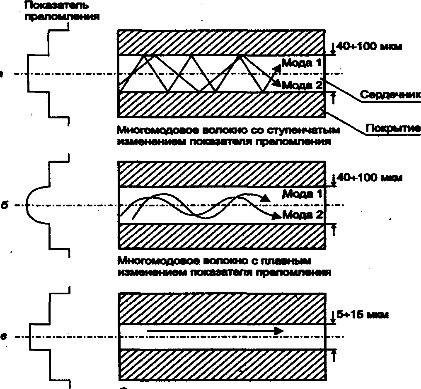
\includegraphics[width=0.5\textwidth]{single-mode-fiber}
    \caption{Одномодовое волокно}
    \label{fig:single-mode-fiber}
\end{figure}

В многомодовых кабелях во внутреннем проводнике одновременно существует несколько световых лучей, отражающихся от внешнего проводника под разными углами.
Угол отражения луча называется модой луча.
В многомодовых кабелях с плавным изменением коэффициента преломления режим распространения каждой моды имеет более сложный характер.

Многомодовые кабели имеют более узкую полосу пропускания - от 500 до 800 МГц/км.
Сужение полосы происходит из-за потерь световой энергии при отражениях, а также из-за интерференции лучей разных мод.

В качестве источников излучения света в волоконно-оптических кабелях применяются:
\begin{itemize}
    \item светодиоды;
    \item полупроводниковые лазеры.
\end{itemize}

Для \emph{одномодовых кабелей} применяются только полупроводниковые лазеры, так как при таком малом диаметре оптического волокна световой поток, создаваемый светодиодом, невозможно без больших потерь направить в волокно.
Для многомодовых кабелей используются более дешевые светодиодные излучатели.

Для передачи информации применяется свет с длиной волны 1550 нм (1,55 мкм), 1300 нм (1,3 мкм) и 850 нм (0,85 мкм).
Светодиоды могут излучить свет с длиной волны 850 нм и 1300 нм.
Лазерные излучатели работают на длинах волн 1300 и 1550 нм.
Лазерные излучатели создают когерентный поток света, за счет чего потери в оптических волокнах становятся меньше, чем при использовании некогерентного потока светодиодов.

Использование только нескольких фиксированных длин волн для передачи информации в оптических волокнах связанно с тем, что именно для этих дискретных длин волн наблюдается минимум потерь.

Волоконно-оптические кабели присоединяют к оборудованию разъемами MIC, SТ и SС.

Волоконно-оптические кабели обладают отличными характеристиками всех типов: электромагнитными, механическими (хорошо гнутся, а в соответствующей изоляции обладают хорошей механической прочностью).
Однако у них есть один серьезный недостаток - сложность соединения волокон с разъемами и между собой при необходимости наращивания длины кабеля, что приводит к удорожанию кабельной системы на основе волоконно-оптических кабелей по сравнению с другими кабельными системами.
